
\chapter{Nonaga's Branching Factor Calculation} \label{branching}
% Review Iterative Deepening Minimax and Alpha-Beta pruning.
% Discuss Zobrist hashing and state reuse.
The number of possible moves in any Nonaga board state is given by the following equation: \\
\begin{equation}
B = \sum_{i=1}^{3} \sum_{j=1}^{P_i} \sum_{k=1}^{T_{i,j}} D_{i,j,k}
\label{eq:branching_factor_detailed}
\end{equation}

Where:
\begin{itemize}
    \item $B$: The total branching factor (number of possible complete turns from the current state).
    \item $i$: The index of the current player's piece ($i \in {1, 2, 3}$).
    \item $P_i$: The total number of valid destinations for piece $i$.
    \item $j$: The index of a specific destination for piece $i$ ($j = 1, 2, \dots, P_i$).
    \item $T_{i,j}$: The number of legally movable tiles, dynamically evaluated \textit{after} piece $i$ has been moved to destination $j$.
    \item $k$: The index of a specific movable tile ($k = 1, 2, \dots, T_{i,j}$).
    \item $D_{i,j,k}$: The number of valid placement destinations for tile $k$, given the board configuration resulting from move $j$.
\end{itemize}
To determine the initial branching factor, the calculation can be simplified by exploiting the symmetrical nature of the board on all 3 axis of the central hexagon. First, $D_{i,j,k}$ is the same for all $i,j,k$. Second, calculating the branching factor for only one piece and then multiplying the result by three results in the branching factor of the position. Third, for each piece two moves yield the same number of movable tiles.\\
Calculating the number of tile moves for 2 piece moves, multiplying one of them by 2 and adding it to the other results in all possible piece and tile moves for one piece and multiplying that number by three results in the branching factor of the position.
\begin{figure}[H]
    \centering
    % --- First Figure ---
    \begin{minipage}{0.49\textwidth}
        \centering
        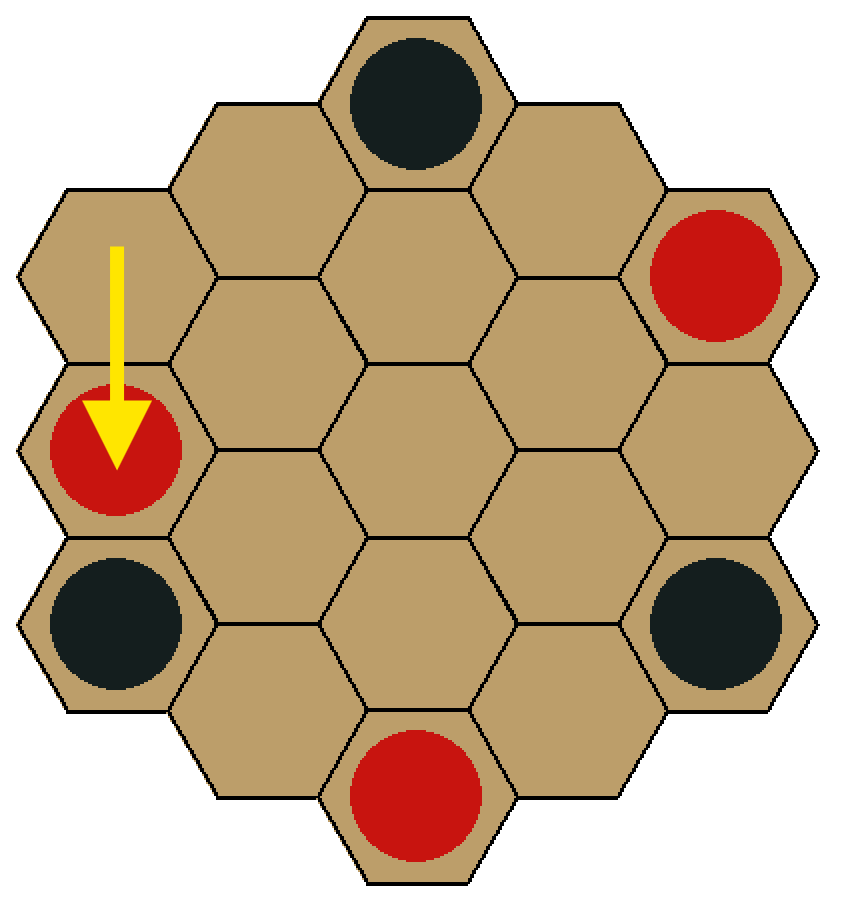
\includegraphics[width=0.42\textwidth]{pictures/init pos/starting piece move to movable.png}
        \caption{Piece move selected.}
        \label{fig:starting piece move to movable}
    \end{minipage}\hfill
    % --- Second Figure ---
    \begin{minipage}{0.49\textwidth}
        \centering
        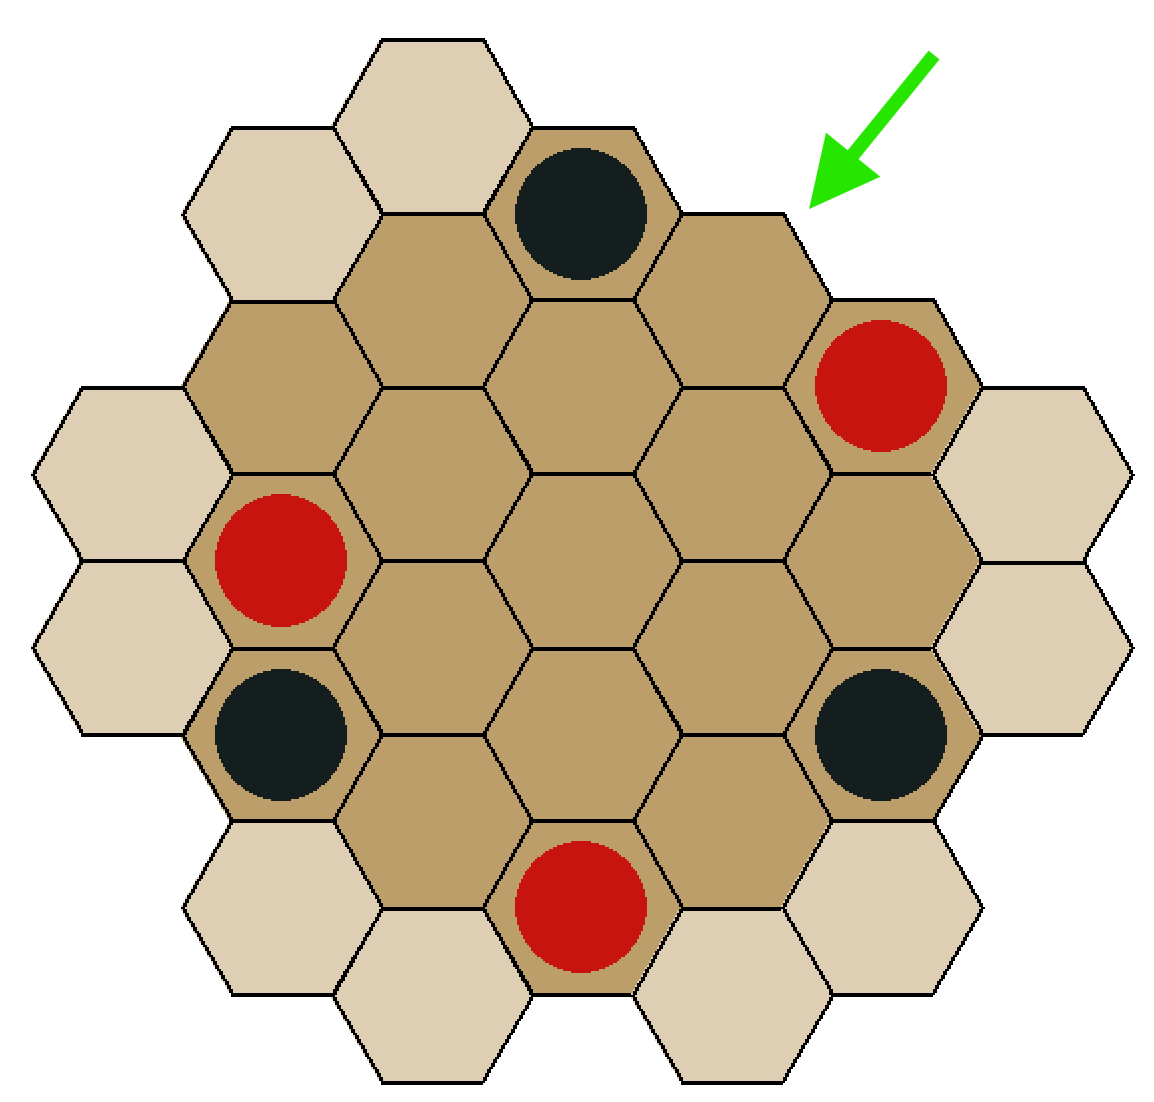
\includegraphics[width=0.58\textwidth]{pictures/init pos/starting tile moves after movable.png}
        \caption{Possible tile moves after the piece move in \cref{fig:starting piece move to movable} of the tile pointed to}
        \label{fig:starting tile moves after movable}
    \end{minipage}
\end{figure}
After the piece move in \cref{fig:starting piece move to movable}, the total number of possible tile moves, as seen in \cref{fig:starting tile moves after movable}, is $NumOfTiles*D = 6*10=60$. It is identical to the total number of possible tile moves after the piece move in \cref{fig:starting piece move to movable 2}. It is doubled to get the number of possible tile moves for both moves.
\begin{figure}[H]
    \centering
    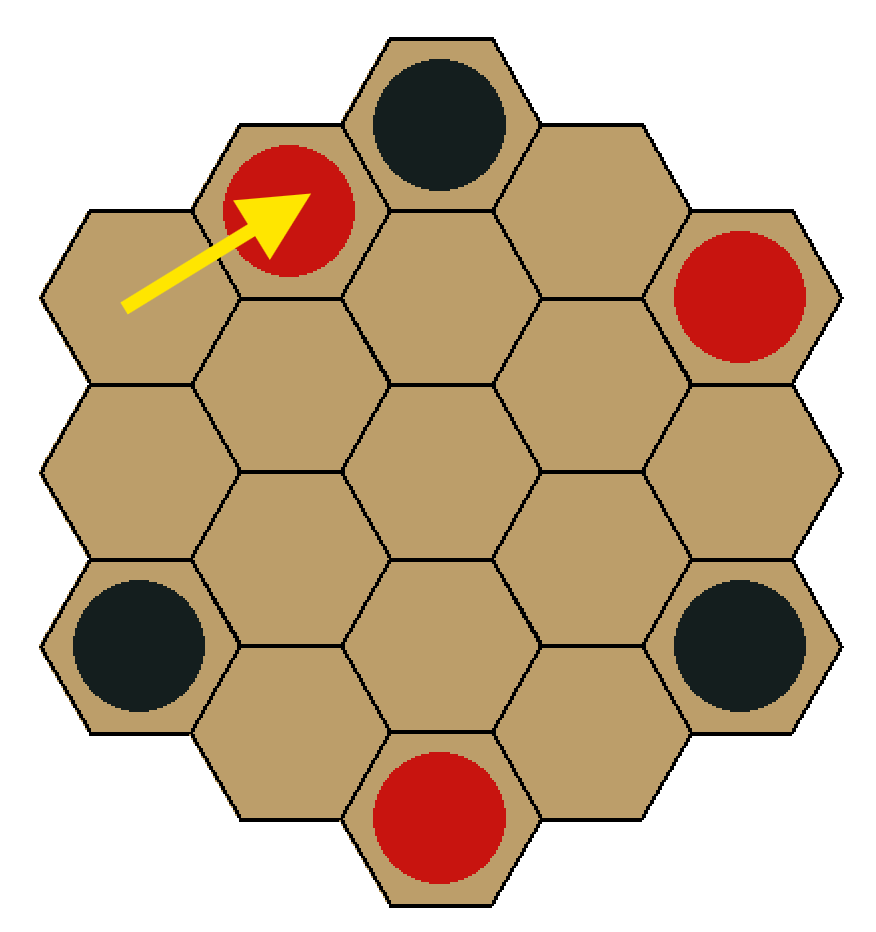
\includegraphics[width=0.235\textwidth]{pictures/init pos/starting piece move to movable 2.png}
    \caption{The piece move with the same number of tile moves as the one in \cref{fig:starting piece move to movable} }
    \label{fig:starting piece move to movable 2}
\end{figure}
\begin{figure}[H]
    \centering
    % --- First Figure ---
    \begin{minipage}{0.45\textwidth}
        \centering
        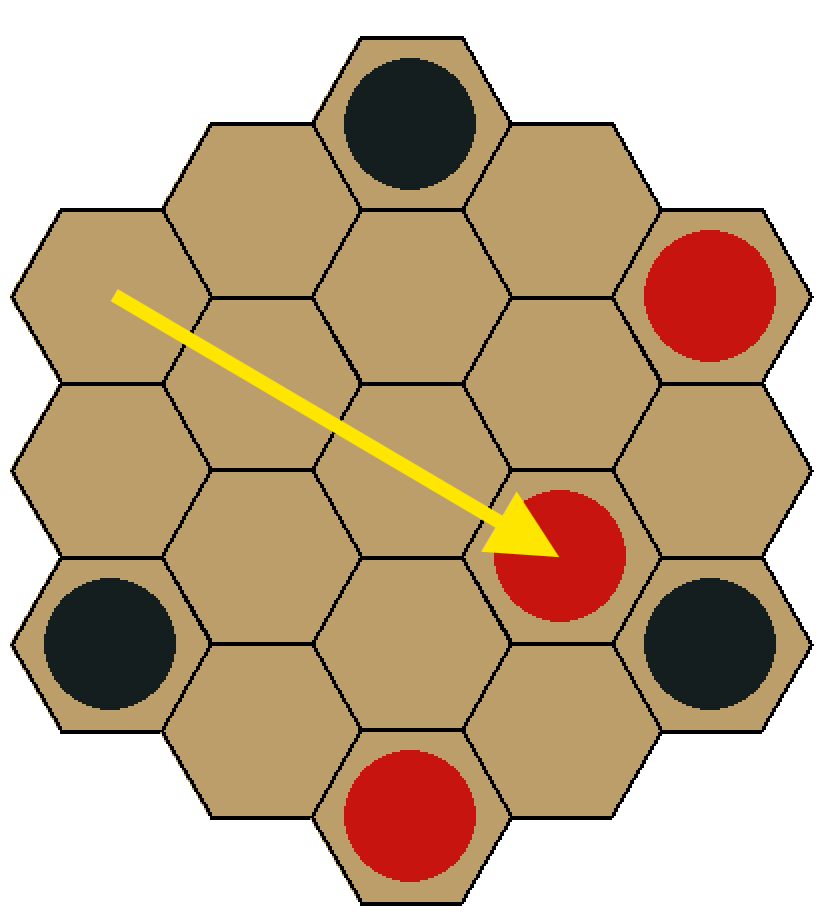
\includegraphics[width=0.43\textwidth]{pictures/init pos/starting piece move to unmovable.png}
        \caption{The last piece move to consider}
        \label{fig:starting piece move to unmovable}
    \end{minipage}\hfill
    % --- Second Figure ---
    \begin{minipage}{0.45\textwidth}
        \centering
        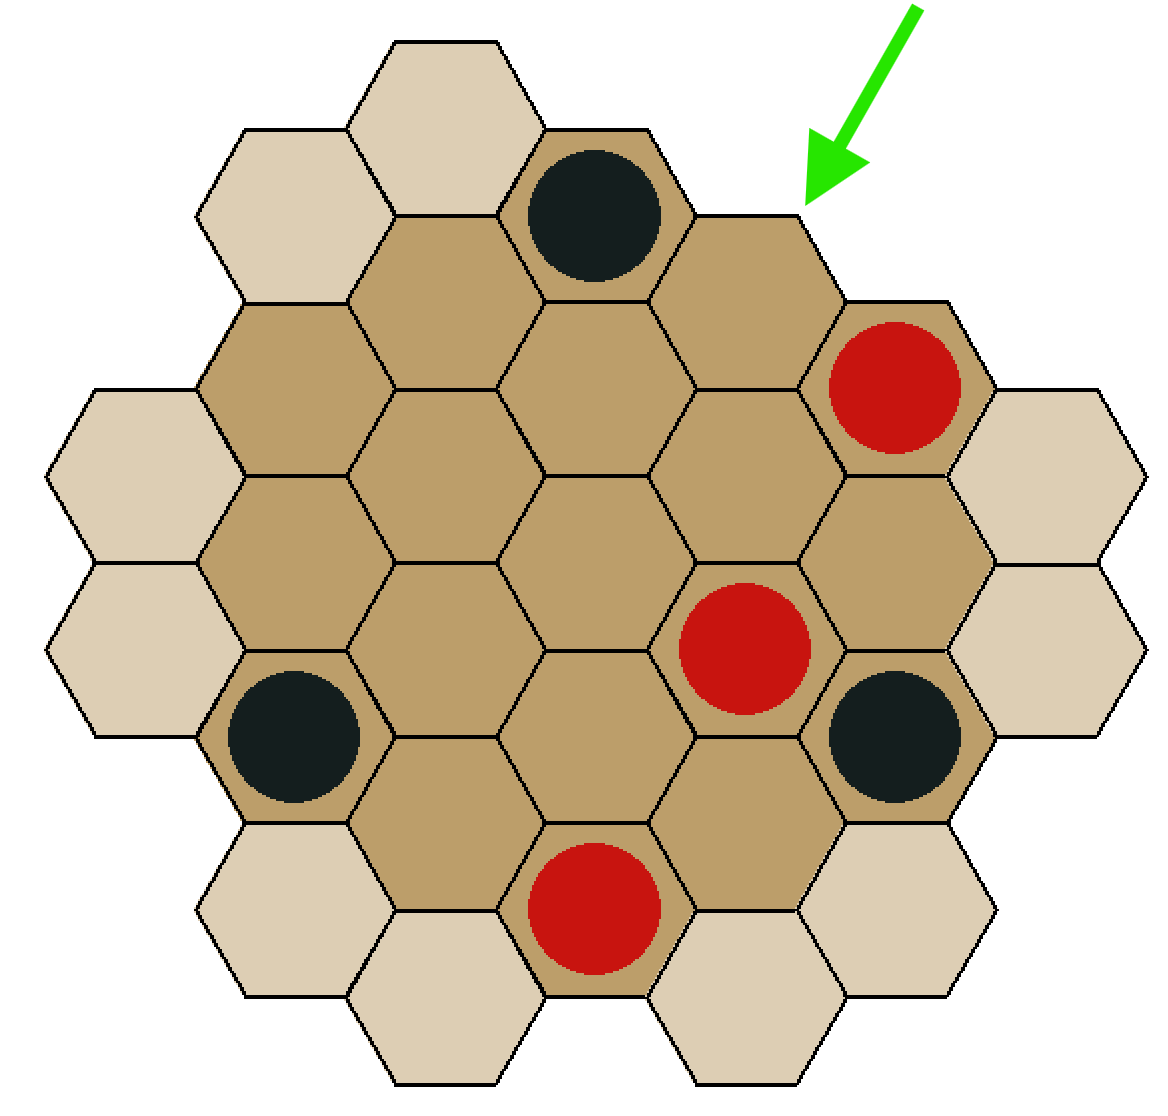
\includegraphics[width=0.60\textwidth]{pictures/init pos/starting tile moves after unmovable.png}
        \caption{Possible tile moves after the piece move in \cref{fig:starting piece move to unmovable} of the tile pointed to}
        \label{fig:starting tile moves after unmovable}
    \end{minipage}
\end{figure}
After the piece move shown in \cref{fig:starting piece move to unmovable}, the total number of possible tile moves (\cref{fig:starting tile moves after unmovable}) is calculated as $N_{\text{tiles}} \times D = 7 \times 10 = 70$. Consequently, the total number of valid moves for the starting position is $3 \times (60 \times 2 + 70) = 570$.While the starting position provides a theoretical maximum, empirical analysis of middle-game states indicates an effective branching factor ($b$) of approximately 440. This reduction occurs because pieces become tightly packed as the game progresses, physically restricting their valid movement vectors.A branching factor of 440 is exceptionally high. For context, Chess has an average branching factor of approximately 35 \cite{Artificial_intelligence}, and Go, a game long considered a grand challenge for AI until the advent of AlphaGo in 2016 \cite{Go_Paper}, averages around 250. However, evaluating a game's computational difficulty requires analyzing the overall game-tree complexity, approximated as $O(b^d)$, where $d$ is the average game depth.While Nonaga's branching factor is roughly 12.5 times larger than that of Chess, a typical game of Nonaga lasts for only about 20 moves. In contrast, Chess averages around 40 full moves (80 plies) and Go extends to roughly 150 moves. Therefore, despite the dense move generation at any individual node, the shallow depth of Nonaga significantly truncates the theoretical search space. 